\subsection{Early-drying risk and a unique-event audit}

\label{sec:rabi_events}

This additional experiment predicts \textbf{new satellite-defined early drying}, not government declarations or independently verified agricultural drought. An event is a post-peak greenness crossing at least 21 days earlier than the point\textquotesingle s historical median drying date. Crop identity and actual harvest dates are not verified. Early drying is therefore a candidate stress signal; it can also reflect crop or management changes. The 2023--2026 seasons were already consulted during development.

\subsubsection{Corrections before the reported run}

The first classifier supplied a completed-season early-drying status as an input, used the validation season in some reference quantities, and included unpublished late-November rainfall at the earliest December issues. Its high status-classification accuracy and repeated-row warning percentages are \textbf{superseded}. Corrected version v2 removes the retrospective status input, builds references only from training seasons, and enforces the eight-day weather cutoff for every weather feature. Its target is an event in $(t,t+h]$, not a status that remains positive after drying.

\subsubsection{Causal inputs and model comparison}

Training uses 2019-20 to 2021-22, validation uses 2022-23, and historical evaluation uses 2023-24 to 2025-26. Each training season is excluded from its own reference. At least two established training seasons with observed drying dates are required. The stricter reference changes the eligible population; v1 and v2 are not a same-cohort ablation. Forecasts use only observations dated at most $t-2$ days, with the latest at most 12 days old, and weather dated at most $t-8$ days. A drying flag observed by issue time is computed from the observation prefix; it is distinct from the retrospective outcome.

Logistic regression, random forest and XGBoost are compared with equal and validation-weighted probability ensembles. Random forest and XGBoost use five seeds; logistic regression is deterministic. The primary model is selected by validation average precision, and thresholds maximize validation balanced accuracy. Baseline imputations, weights and thresholds never use evaluation data. Tables report the seed-averaged deployment predictions; the reproducibility files retain seed metrics.

\begin{figure}[H]

\centering

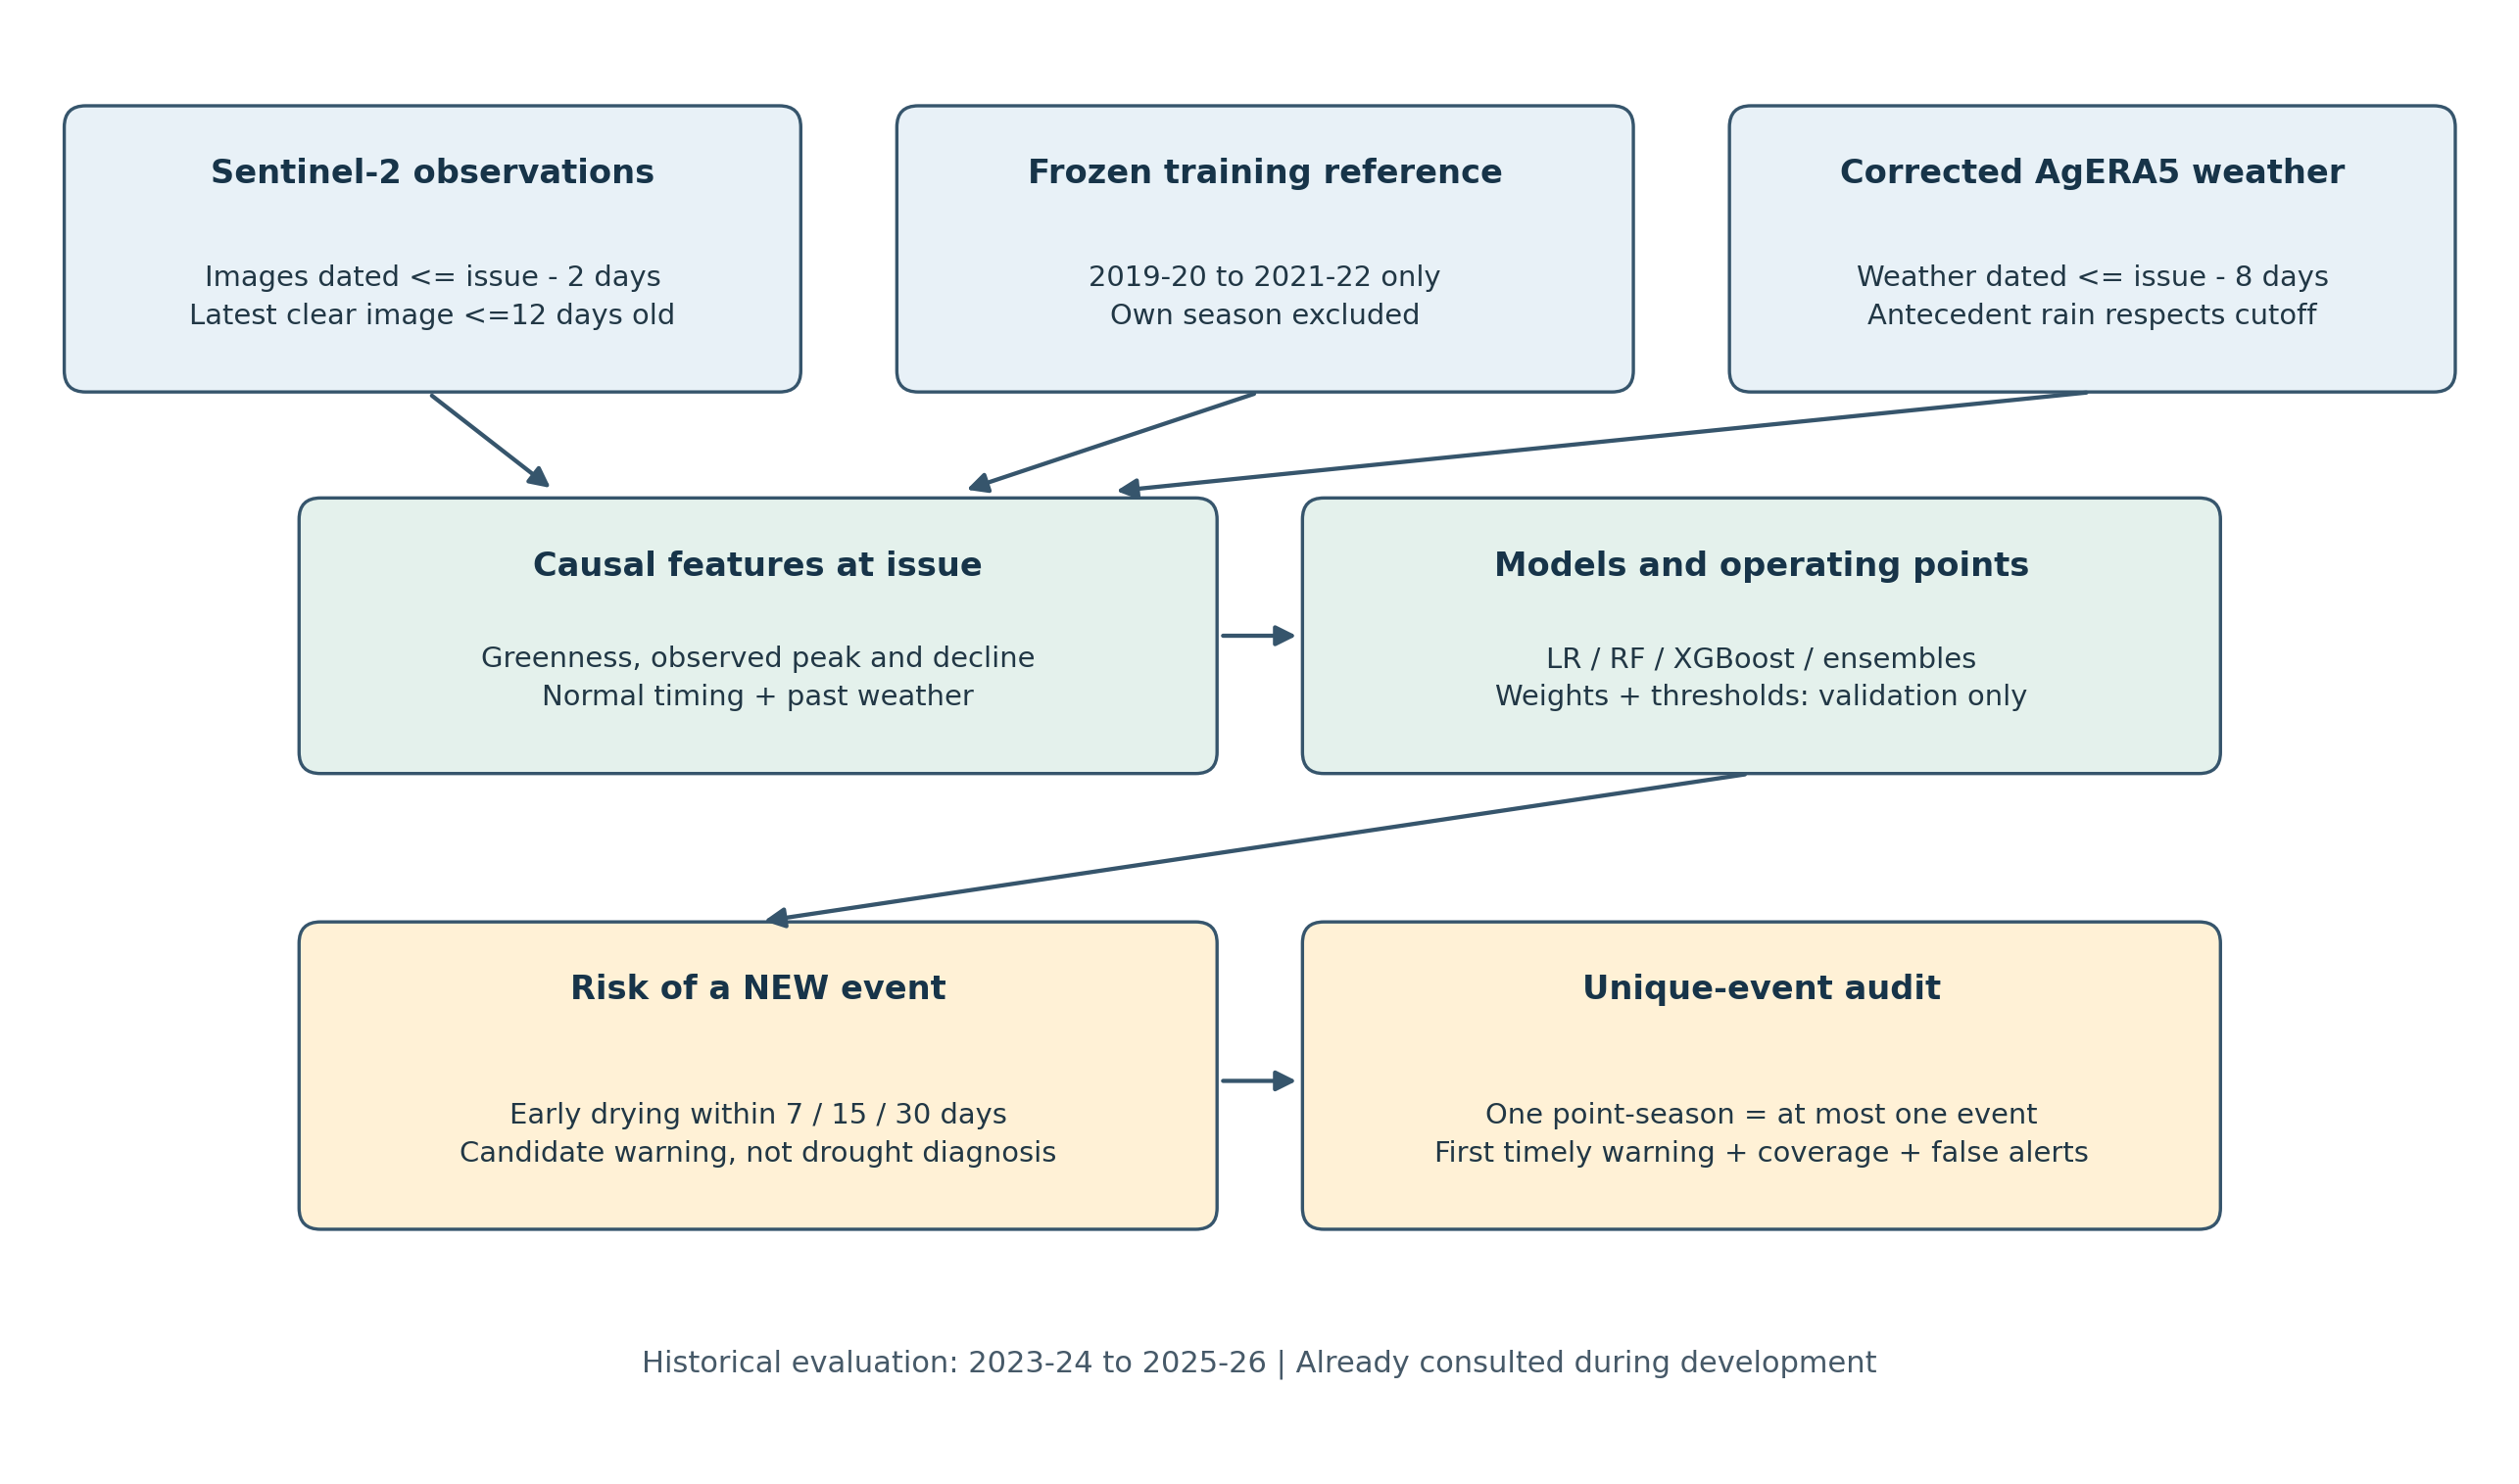
\includegraphics[width=0.98\textwidth]{figures/fig8_rabi_early_drying_architecture.png}

\caption{Corrected rabi early-drying risk workflow. Retrospective labels are used for scoring, not as inputs.}

\label{fig:rabi_event_arch}

\end{figure}

\begin{table}[H]
\centering
\footnotesize
\caption{Reference and observation coverage for the corrected experiment. Points are sampled locations, not verified field boundaries.}
\label{tab:r_event_coverage}
\begin{tabularx}{\textwidth}{@{}Xrrrr@{}}
\toprule
\textbf{Season} & \textbf{Reference eligible} & \textbf{Scorable} & \textbf{Forecast points} & \textbf{Early events} \\
\midrule
2019-20 & 127 & 127 & 92 & 27 \\
2020-21 & 141 & 141 & 96 & 9 \\
2021-22 & 132 & 132 & 103 & 16 \\
2022-23 & 232 & 232 & 149 & 18 \\
2023-24 & 232 & 232 & 148 & 59 \\
2024-25 & 232 & 232 & 161 & 33 \\
2025-26 & 232 & 232 & 145 & 17 \\
\bottomrule
\end{tabularx}
\end{table}


\subsubsection{New-onset point-date performance}

Only forecasts preceding the retrospective event and without an issue-time observed drying flag enter this comparison. These are correlated point-dates, not independent events. Average precision (AP) is reported alongside ROC-AUC because new onsets are uncommon.

\begin{table}[H]
\centering
\footnotesize
\caption{New-onset point-date scores for models selected on validation. Precision and recall are percentages.}
\label{tab:r_onset_metrics}
\begin{tabularx}{\textwidth}{@{}rXrrrrr@{}}
\toprule
\textbf{Days} & \textbf{Selected model} & \textbf{Rows (positive)} & \textbf{AUC} & \textbf{AP} & \textbf{Precision} & \textbf{Recall} \\
\midrule
7 & Random forest & 6833 (144) & 0.925 & 0.175 & 7.5 & 95.8 \\
15 & Random forest & 6833 (292) & 0.914 & 0.312 & 16.2 & 89.7 \\
30 & Random forest & 6833 (527) & 0.905 & 0.372 & 24.2 & 92.0 \\
\bottomrule
\end{tabularx}
\end{table}


\subsubsection{One count per drying event}

An event is one sampled point-season with an observed early-drying date. For horizon $h$, a timely warning must precede the event by more than zero and no more than $h$ days. Repeated warnings cannot increase the count of caught events. The denominator includes all monitored events, including events without a usable advance observation. Opportunity recall is additionally reported in the source tables.

Warning precision in Table~\ref{tab:r_unique_events} is the fraction of \emph{warned point-seasons} with at least one timely warning. A point-season with earlier false alerts and a later timely alert counts once as successful, so this is not per-alert precision. Table~\ref{tab:r_onset_metrics} retains the point-date precision. Lead time uses the first timely warning for each caught event, once.

\begin{table}[H]
\centering
\footnotesize
\caption{Unique early-drying events. Recall uses all monitored events; precision uses warned point-seasons. Lead is the median first timely warning.}
\label{tab:r_unique_events}
\begin{tabularx}{\textwidth}{@{}rXrrrrr@{}}
\toprule
\textbf{Days} & \textbf{Selected model} & \textbf{Caught / events} & \textbf{With opportunity} & \textbf{Recall (\%)} & \textbf{Precision (\%)} & \textbf{Lead (d)} \\
\midrule
7 & Random forest & 102 / 108 & 104 & 94.4 & 30.8 & 5 \\
15 & Random forest & 101 / 108 & 106 & 93.5 & 33.1 & 12 \\
30 & Random forest & 104 / 108 & 107 & 96.3 & 31.3 & 27 \\
\bottomrule
\end{tabularx}
\end{table}


\begin{table}[H]
\centering
\footnotesize
\caption{Recall requiring a minimum useful lead, among all monitored early-drying events (percent).}
\label{tab:r_useful_lead}
\begin{tabularx}{\textwidth}{@{}Xrrr@{}}
\toprule
\textbf{Days} & \textbf{At least 7 d lead} & \textbf{At least 14 d lead} & \textbf{Lead IQR (d)} \\
\midrule
7 & 21.3 & 0.0 & 3--6 \\
15 & 84.3 & 12.0 & 11--13 \\
30 & 91.7 & 83.3 & 20--28 \\
\bottomrule
\end{tabularx}
\end{table}


\subsubsection{Uncertainty and interpretation}

\begin{table}[H]
\centering
\footnotesize
\caption{95\% bootstrap intervals for unique-event recall and warned-point-season precision. Cell intervals are indicative with very few clusters.}
\label{tab:r_event_ci}
\begin{tabularx}{\textwidth}{@{}rXrrr@{}}
\toprule
\textbf{Days} & \textbf{Resampling unit} & \textbf{Clusters} & \textbf{Recall interval (\%)} & \textbf{Precision interval (\%)} \\
\midrule
7 & point\_id & 232 & 89.7--98.1 & 25.3--36.1 \\
7 & cell & 5 & 84.6--97.4 & 25.2--36.5 \\
15 & point\_id & 232 & 88.5--97.6 & 27.5--38.7 \\
15 & cell & 5 & 90.0--94.7 & 27.7--39.2 \\
30 & point\_id & 232 & 92.2--99.2 & 25.9--37.0 \\
30 & cell & 5 & 94.4--98.4 & 26.7--37.2 \\
\bottomrule
\end{tabularx}
\end{table}


The event ledger and full model/baseline tables are saved under \texttt{rabi\_module/results/detect\_v2/}; operating points and validation predictions are retained. Rainfall association is a descriptive cell-season consistency check, not independent field validation. The reference spans only two or three seasons, and cloud gaps and retrospective smoothing make the crossing date an image-based estimate rather than a measured physiological onset. No observed crossing does not prove a crop was free of water stress. Before claiming drought detection, alerts require independent evidence on crop water stress and crop-management timing.



\subsubsection{Rainfall association}

The corrected reference yields 21 cell-seasons with at least ten established points. The Spearman correlation of early-drying share with June--November rain relative to normal is -0.423. This is descriptive historical association, not causal or field-level validation. There are 0 qualifying cell-seasons below 80\,\% of normal rain, so the low-rain versus other-years rate contrast cannot be estimated under that rule. The previous ``twice as common statement is not carried forward to this corrected cohort.

\subsubsection{Always-warn sanity check}

This diagnostic was added after viewing the primary v2 results and did not change any model, threshold or selection. Warning at every usable issue also catches almost all events. Thus event recall and first-timely lead cannot be interpreted without the warning burden. The learned model reduces alerts, but many warned point-seasons still have no timely event.

\begin{table}[H]
\centering
\footnotesize
\caption{Selected model versus warning at every usable issue. One warned unit is one point-season. This diagnostic is not used to choose the model.}
\label{tab:r_always_warn}
\begin{tabularx}{\textwidth}{@{}Xrrrr@{}}
\toprule
\textbf{Days} & \textbf{Model caught} & \textbf{Always caught} & \textbf{Model warned} & \textbf{Always warned} \\
\midrule
7 & 102/108 & 104/108 & 331 & 453 \\
15 & 101/108 & 106/108 & 305 & 453 \\
30 & 104/108 & 107/108 & 332 & 453 \\
\bottomrule
\end{tabularx}
\end{table}
